
\begin{frame}{Removing particle}
  We remove a particle at \textbf{position x} with a spin $\sigma$
  \begin{equation*}
    \ket{\phi_\sigma(\x)} = \hat{\psi}_\sigma(\x)\ket{g}
  \end{equation*}

  \vspace{0.5cm}
  Particle density at this state:
  \begin{equation*}
    \rho(\x', \sigma') = \bra{\phi_\sigma(\x)}\hat{\psi}_{\sigma'}^\dagger(\x')\hat{\psi}_{\sigma'}(\x')\ket{\phi_\sigma(\x)}
  \end{equation*}

  \vspace{0.5cm}
  We will show that the density equals to
  \only<1>{
  \begin{equation*}
    \left ( \frac{N}{2\V}\right )^2 \: g_{\sigma \sigma'}(\x - \x')
  \end{equation*}
  }
  \only<2>{
  \begin{equation*}
    \textcolor{red}{\left ( \frac{N}{2\V}\right )^2} \: g_{\sigma \sigma'}(\x - \x')
  \end{equation*}
  }
  \only<3>{
  \begin{equation*}
    \left ( \frac{N}{2\V}\right )^2 \: \textcolor{red}{g_{\sigma \sigma'}(\x - \x')}
  \end{equation*}
  }

\end{frame}

\begin{frame}{Removing particle}
  The state after removing a particle. In coordinate space:
  \begin{equation*}
    \ket{\phi_\sigma(\x)} = \hat{\psi}_\sigma(\x)\ket{g}
  \end{equation*}

  But we want to use momentum space:

  \begin{block}{Fourier tranform}
    $$\hat{\psi}_{\veck, \sigma}(\x) = \sum_{\veck} \hat{c}_{\veck,\sigma} \psi_{\veck,\sigma}(\x)$$
  \end{block}
  \begin{equation*}
    \begin{gathered}
      \psi_{\veck, \sigma}(\x) = \frac{1}{\sqrt{\V}} e^{i\veck \cdot \x} \: \boldsymbol{\sigma}
    \end{gathered}
  \end{equation*}

\end{frame}

\begin{frame}{Density in momentum space}
  \only<1>{
  \begin{equation*}
    \begin{gathered}
      \rho(\x', \sigma') =\\
       \bra{g} \sum_{\veck} \hat{c}_{\veck,\sigma}^{\dagger} \psi_{\veck,\sigma}^\ast(\x)
      \sum_{\textbf{l}} \hat{c}_{\textbf{l},\sigma'}^\dagger \psi_{\textbf{l},\sigma'}^\ast (\x')
      \sum_{\textbf{m}} \hat{c}_{\textbf{m},\sigma'} \psi_{\textbf{m},\sigma'} (\x')
      \sum_{\textbf{n}} \hat{c}_{\textbf{n},\sigma} \psi_{\textbf{n},\sigma} (\x) \ket{g} =\\
      \sum_{\veck, \textbf{l}, \textbf{m}, \textbf{n}}
      \bra{g} \hat{c}_{\veck,\sigma}^{\dagger}  \hat{c}_{\textbf{l},\sigma'}^\dagger
      \hat{c}_{\textbf{m},\sigma'} \hat{c}_{\textbf{n},\sigma} \ket{g}
      \psi_{\veck,\sigma}^\ast(\x) \psi_{\textbf{l},\sigma'}^\ast (\x')
       \psi_{\textbf{m},\sigma'} (\x') \psi_{\textbf{n},\sigma} (\x)
    \end{gathered}
  \end{equation*}
  }
  \only<2>{
  \begin{equation*}
    \begin{gathered}
      \rho(\x', \sigma') =\\
       \bra{g} \sum_{\veck} \hat{c}_{\veck,\sigma}^{\dagger} \psi_{\veck,\sigma}^\ast(\x)
      \sum_{\textbf{l}} \hat{c}_{\textbf{l},\sigma'}^\dagger \psi_{\textbf{l},\sigma'}^\ast (\x')
      \sum_{\textbf{m}} \hat{c}_{\textbf{m},\sigma'} \psi_{\textbf{m},\sigma'} (\x')
      \sum_{\textbf{n}} \hat{c}_{\textbf{n},\sigma} \psi_{\textbf{n},\sigma} (\x) \ket{g} =\\
      \sum_{\veck, \textbf{l}, \textbf{m}, \textbf{n}}
      \textcolor{red}{\bra{g} \hat{c}_{\veck,\sigma}^{\dagger}  \hat{c}_{\textbf{l},\sigma'}^\dagger
      \hat{c}_{\textbf{m},\sigma'} \hat{c}_{\textbf{n},\sigma} \ket{g} }
      \psi_{\veck,\sigma}^\ast(\x) \psi_{\textbf{l},\sigma'}^\ast (\x')
       \psi_{\textbf{m},\sigma'} (\x') \psi_{\textbf{n},\sigma} (\x)
    \end{gathered}
  \end{equation*}
  }
\end{frame}

\begin{frame}[t]{Allowed operators}
  \vspace{0.3cm}
  We will focus on the expression
  \begin{equation*}
    \bra{g} \hat{c}_{\veck,\sigma}^{\dagger}  \hat{c}_{\textbf{l},\sigma'}^\dagger
    \hat{c}_{\textbf{m},\sigma'} \hat{c}_{\textbf{n},\sigma} \ket{g}
  \end{equation*}

  \vspace{0.2cm}

  \only<1>{
  Removing two particles:
  \begin{equation*}
    \ket{g}
  \end{equation*}

  \begin{figure}
    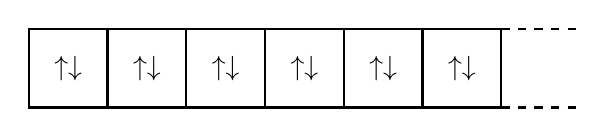
\begin{tikzpicture}
      \foreach \xbox in {0, ..., 5} {
        \def\ybox{0}
        \node at (\xbox+0.5,\ybox+0.5) {$\uparrow \downarrow$};
        \path[draw,thick] (\xbox,\ybox) rectangle (\xbox+1,\ybox+1);
      }
      \path[draw,dashed,thick] (6,0) -- (7,0) (6,1) -- (7,1);
    \end{tikzpicture}
  \end{figure}
  }

  \only<2>{
  Removing two particles:
  \begin{equation*}
    \hat{c}_{\textbf{n},\sigma} \ket{g}
  \end{equation*}

  \begin{figure}
    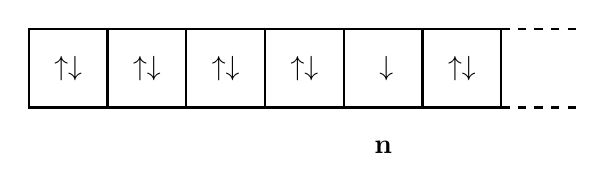
\begin{tikzpicture}
      \foreach \xbox in {0, ..., 3} {
        \def\ybox{0}
        \node at (\xbox+0.5,\ybox+0.5) {$\uparrow \downarrow$};
        \path[draw,thick] (\xbox,\ybox) rectangle (\xbox+1,\ybox+1);
      }

      \def\xbox{4}
      \node at (\xbox+0.5,0+0.5) {$\: \downarrow$};
      \path[draw,thick] (\xbox,0) rectangle (\xbox+1,0+1);
      \node at (\xbox+0.5,0-0.5) {\textbf{n}};

      \def\xbox{5}
      \node at (\xbox+0.5,0+0.5) {$\uparrow \downarrow$};
      \path[draw,thick] (\xbox,0) rectangle (\xbox+1,0+1);

      \path[draw,dashed,thick] (6,0) -- (7,0) (6,1) -- (7,1);
    \end{tikzpicture}
  \end{figure}
  }

  \only<3>{
  Removing two particles:
  \begin{equation*}
    \hat{c}_{\textbf{m},\sigma'} \hat{c}_{\textbf{n},\sigma} \ket{g}
  \end{equation*}

  \begin{figure}
    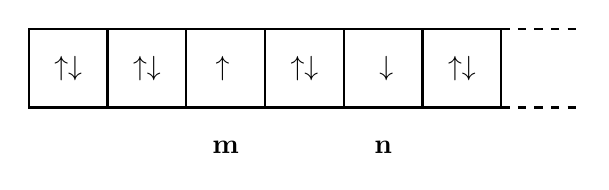
\begin{tikzpicture}
      \foreach \xbox in {0, ..., 1} {
        \def\ybox{0}
        \node at (\xbox+0.5,\ybox+0.5) {$\uparrow \downarrow$};
        \path[draw,thick] (\xbox,\ybox) rectangle (\xbox+1,\ybox+1);
      }

      \def\xbox{2}
      \node at (\xbox+0.5,0+0.5) {$\uparrow \:$};
      \path[draw,thick] (\xbox,0) rectangle (\xbox+1,0+1);
      \node at (\xbox+0.5,0-0.5) {\textbf{m}};

      \def\xbox{3}
      \node at (\xbox+0.5,0+0.5) {$\uparrow \downarrow$};
      \path[draw,thick] (\xbox,0) rectangle (\xbox+1,0+1);

      \def\xbox{4}
      \node at (\xbox+0.5,0+0.5) {$\: \downarrow$};
      \path[draw,thick] (\xbox,0) rectangle (\xbox+1,0+1);
      \node at (\xbox+0.5,0-0.5) {\textbf{n}};

      \def\xbox{5}
      \node at (\xbox+0.5,0+0.5) {$\uparrow \downarrow$};
      \path[draw,thick] (\xbox,0) rectangle (\xbox+1,0+1);

      \path[draw,dashed,thick] (6,0) -- (7,0) (6,1) -- (7,1);
    \end{tikzpicture}
  \end{figure}
  }

  \only<4>{
  Restoring the state:
  \begin{equation*}
    \hat{c}_{\veck,\sigma}^{\dagger}  \hat{c}_{\textbf{l},\sigma'}^\dagger
    \hat{c}_{\textbf{m},\sigma'} \hat{c}_{\textbf{n},\sigma} \ket{g}
  \end{equation*}
  \begin{figure}
    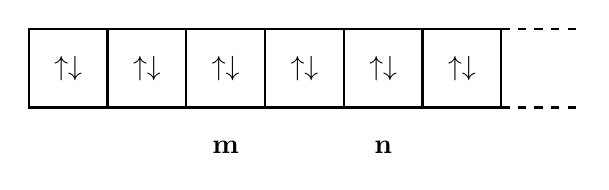
\begin{tikzpicture}
      \foreach \xbox in {0, ..., 5} {
        \def\ybox{0}
        \node at (\xbox+0.5,\ybox+0.5) {$\uparrow \downarrow$};
        \path[draw,thick] (\xbox,\ybox) rectangle (\xbox+1,\ybox+1);
      }
      \node at (2+0.5,0-0.5) {\textbf{m}};
      \node at (4+0.5,0-0.5) {\textbf{n}};
      \path[draw,dashed,thick] (6,0) -- (7,0) (6,1) -- (7,1);
    \end{tikzpicture}
  \end{figure}
  }

  \only<5>{
  \begin{block}{Allowed indices}
    \begin{equation*}
      \begin{gathered}
        \begin{cases} \textbf{k}, \sigma = \textbf{m}, \sigma'\\
          \textbf{l}, \sigma' = \textbf{n}, \sigma \end{cases}
          \qquad
          \begin{cases}   \textbf{k}, \sigma = \textbf{n}, \sigma\\
            \textbf{l}, \sigma' = \textbf{m}, \sigma' \end{cases}
      \end{gathered}
    \end{equation*}
  \end{block}
  }
\end{frame}

\begin{frame}[t]{Density for different spin}
  \vspace{0.3cm}
  If spins are different
  \begin{equation*}
    \sigma \ne \sigma' \implies \text{ only } \begin{cases}   \textbf{k} = \textbf{n}\\
      \textbf{l} = \textbf{m} \end{cases}
  \end{equation*}

  We can simplify expression for density:
  \only<1,2>{
  \begin{equation*}
    \begin{gathered}
      \rho(\x', \sigma') =
      \sum_{\veck, \textbf{l}}
      \bra{g} \hat{c}_{\veck,\sigma}^{\dagger}  \hat{c}_{\textbf{l},\sigma'}^\dagger
      \hat{c}_{\textbf{l},\sigma'} \hat{c}_{\textbf{k},\sigma} \ket{g}
      \psi_{\veck,\sigma}^\ast(\x) \psi_{\textbf{l},\sigma'}^\ast (\x')
       \psi_{\textbf{l},\sigma'} (\x') \psi_{\textbf{k},\sigma} (\x)
    \end{gathered}
  \end{equation*}
  }

  \only<3>{
  \begin{equation*}
    \begin{gathered}
      \rho(\x', \sigma') = \frac{1}{\V}
      \sum_{\veck, \textbf{l}}
      \bra{g} \hat{c}_{\veck,\sigma}^{\dagger}  \hat{c}_{\textbf{l},\sigma'}^\dagger
      \hat{c}_{\textbf{l},\sigma'} \hat{c}_{\textbf{k},\sigma} \ket{g}
      \psi_{\veck,\sigma}^\ast(\x) \psi_{\textbf{k},\sigma} (\x)
    \end{gathered}
  \end{equation*}
  }

  \only<4>{
  \begin{equation*}
    \begin{gathered}
      \rho(\x', \sigma') = \frac{1}{\V^2}
      \sum_{\veck, \textbf{l}}
      \bra{g} \hat{c}_{\veck,\sigma}^{\dagger}  \hat{c}_{\textbf{l},\sigma'}^\dagger
      \hat{c}_{\textbf{l},\sigma'} \hat{c}_{\textbf{k},\sigma} \ket{g}
    \end{gathered}
  \end{equation*}
  }

  \only<2>{
  \begin{block}{Wave functions}
    \begin{equation*}
      \begin{gathered}
        \psi_{\textbf{l},\sigma'}(\x') = \frac{1}{\sqrt{\V}} e^{i\textbf{l}\cdot \x'} \: \boldsymbol{\sigma'}\\
        \psi_{\textbf{l},\sigma'}^\ast(\x') = \frac{1}{\sqrt{\V}} e^{-i\textbf{l}\cdot \x'} \: \boldsymbol{\sigma'}
      \end{gathered}
    \end{equation*}
  \end{block}
  }
\end{frame}

\begin{frame}[t]{Density for different spin}
  \vspace{0.3cm}
  If spins are different
  \begin{equation*}
    \sigma \ne \sigma' \implies \text{ only } \begin{cases}   \textbf{k} = \textbf{n}\\
      \textbf{l} = \textbf{m} \end{cases}
  \end{equation*}

  We can simplify expression for density:
  \only<1>{
  \begin{equation*}
    \begin{gathered}
      \rho(\x', \sigma') = \frac{1}{\V^2}
      \sum_{\veck, \textbf{l}}
      \bra{g} \hat{c}_{\veck,\sigma}^{\dagger}  \hat{c}_{\textbf{l},\sigma'}^\dagger
      \hat{c}_{\textbf{l},\sigma'} \hat{c}_{\textbf{k},\sigma} \ket{g}
    \end{gathered}
  \end{equation*}
  }

  \only<2,3>{
  \begin{equation*}
    \begin{gathered}
      \rho(\x', \sigma') = \frac{-1}{\V^2}
      \sum_{\veck, \textbf{l}}
      \bra{g} \hat{c}_{\veck,\sigma}^{\dagger}  \hat{c}_{\textbf{l},\sigma'}^\dagger
      \hat{c}_{\textbf{k},\sigma} \hat{c}_{\textbf{l},\sigma'} \ket{g}
    \end{gathered}
  \end{equation*}
  }

  \only<4>{
  \begin{equation*}
    \begin{gathered}
      \rho(\x', \sigma') = \frac{1}{\V^2}
      \sum_{\veck, \textbf{l}}
      \bra{g} \hat{c}_{\veck,\sigma}^{\dagger} \hat{c}_{\textbf{k},\sigma}
      \hat{c}_{\textbf{l},\sigma'}^\dagger \hat{c}_{\textbf{l},\sigma'} \ket{g} - \\
      - \delta_{\sigma,\sigma'}\frac{1}{\V^2}\sum_{\veck}
      \bra{g}\hat{c}_{\veck,\sigma}^{\dagger} \hat{c}_{\textbf{k},\sigma}\ket{g}
    \end{gathered}
  \end{equation*}
  }

  \only<1,2>{
  \begin{block}{Commutation for fermions}
    \begin{equation*}
      \{ \hat{c}_{\textbf{l},\sigma'} \hat{c}_{\textbf{k},\sigma} \} = 0 \implies
      \hat{c}_{\textbf{l},\sigma'} \hat{c}_{\textbf{k},\sigma} =
      - \hat{c}_{\textbf{k},\sigma} \hat{c}_{\textbf{l},\sigma'}
    \end{equation*}
  \end{block}
  }

  \only<3,4>{
  \begin{block}{Commutation for fermions}
    \begin{equation*}
      \{ \hat{c}_{\textbf{l},\sigma'}^\dagger \hat{c}_{\textbf{k},\sigma} \} = \delta_{k,l} \implies
      \hat{c}_{\textbf{l},\sigma'}^\dagger \hat{c}_{\textbf{k},\sigma} =
      - \hat{c}_{\textbf{k},\sigma} \hat{c}_{\textbf{l},\sigma'}^\dagger + \delta_{k,l}
    \end{equation*}
  \end{block}
  }

\end{frame}


\begin{frame}[t]{Density for different spin}
  \vspace{0.6cm}
  Insert identity operator:
  \only<1,2>{
  \begin{equation*}
    \begin{gathered}
      \rho(\x', \sigma') = \frac{1}{\V^2}
      \sum_{\veck, \textbf{l}}
      \bra{g} \hat{c}_{\veck,\sigma}^{\dagger} \hat{c}_{\textbf{k},\sigma} \: \hat{\mathcal{I}} \:
      \hat{c}_{\textbf{l},\sigma'}^\dagger \hat{c}_{\textbf{l},\sigma'} \ket{g}
    \end{gathered}
  \end{equation*}
  }

  \only<3>{
  \begin{equation*}
    \begin{gathered}
      \rho(\x', \sigma') = \frac{1}{\V^2}
      \sum_{\veck, \textbf{l}}
      \bra{g} \hat{c}_{\veck,\sigma}^{\dagger} \hat{c}_{\textbf{k},\sigma} \: \sum_{n}\ket{n}\bra{n} \:
      \hat{c}_{\textbf{l},\sigma'}^\dagger \hat{c}_{\textbf{l},\sigma'} \ket{g}
    \end{gathered}
  \end{equation*}
  }

  \only<4,5>{
  \begin{equation*}
    \begin{gathered}
      \rho(\x', \sigma') = \frac{1}{\V^2}
      \sum_{\veck, \textbf{l}}
      \bra{g} \hat{c}_{\veck,\sigma}^{\dagger} \hat{c}_{\textbf{k},\sigma} \ket{g}\:\bra{g}
      \hat{c}_{\textbf{l},\sigma'}^\dagger \hat{c}_{\textbf{l},\sigma'} \ket{g}
    \end{gathered}
  \end{equation*}
  }

  \only<2,3>{
  \begin{block}{Identuty}
    \begin{equation*}
      \hat{\mathcal{I}} = \sum_{n}\ket{n}\bra{n}
    \end{equation*}
  \end{block}
  }

  \only<3,4>{
  \begin{block}{Fock space}
    \begin{equation*}
      \bra{n}\ket{g} = \delta_{n,g}
    \end{equation*}
  \end{block}
  }
  \only<4,5>{
  \begin{block}{Number of particles operator}
    $$ \hat c^{\dagger}_{\textbf{k}\sigma} \hat c_{\textbf{k}\sigma} = \hat n_{\textbf{k}\sigma}$$
  \end{block}
  }
  \only<5>{
  \begin{equation*}
    \begin{gathered}
      \rho(\x', \sigma') = \frac{1}{\V^2}
      \left [ \sum_{\veck} \bra{g} \hat n_{\textbf{k}\sigma} \ket{g} \right ] \cdot
      \left [  \sum_{\textbf{l}} \bra{g} \hat n_{\textbf{l}\sigma'} \ket{g} \right ]
      =   \left ( \frac{N}{2\V}\right )^2
    \end{gathered}
  \end{equation*}
  }
\end{frame}

\begin{frame}[t]{Density for equal spin}
\vspace{0.6cm}
 If spins are equal
  \begin{equation*}
    \sigma = \sigma' \implies \text{ only } \begin{cases}   \textbf{k} = \textbf{m}\\
      \textbf{l} = \textbf{n} \end{cases}
  \end{equation*}

  We can simplify expression for density:
  \only<1,2>{
  \begin{equation*}
    \begin{gathered}
      \rho(\x', \sigma) =
      \sum_{\veck, \textbf{l}}
      \bra{g} \hat{c}_{\veck\sigma}^{\dagger}   \hat{c}_{\textbf{l}\sigma}^\dagger \hat{c}_{\textbf{k}\sigma} \hat{c}_{\textbf{l}\sigma} \ket{g}
      \psi_{\veck\sigma}^\ast(\x)
       \psi_{\textbf{l}\sigma}^\ast (\x') \psi_{\textbf{k}\sigma} (\x') \psi_{\textbf{l}\sigma} (\x)
    \end{gathered}
  \end{equation*}
  }

  \only<3>{
    \begin{equation*}
    \begin{gathered}
      \rho(\x', \sigma) =
      -\sum_{\veck, \textbf{l}}
      \bra{g} \hat{c}_{\veck\sigma}^{\dagger} \hat{c}_{\textbf{k}\sigma}  \hat{c}_{\textbf{l}\sigma}^\dagger  \hat{c}_{\textbf{l}\sigma} \ket{g}
      \psi_{\veck\sigma}^\ast(\x) \psi_{\textbf{k}\sigma} (\x')
       \psi_{\textbf{l}\sigma}^\ast (\x') \psi_{\textbf{l}\sigma} (\x)
    \end{gathered}
  \end{equation*}
  }

  \only<4>{
  \begin{equation*}
    \begin{gathered}
      \rho(\x', \sigma) = -\frac{1}{\V^2}
      \sum_{\veck, \textbf{l}}
      \bra{g} \hat{c}_{\veck\sigma}^{\dagger} \hat{c}_{\textbf{k}\sigma}  \hat{c}_{\textbf{l}\sigma}^\dagger  \hat{c}_{\textbf{l}\sigma} \ket{g}
      e^{-i\vec{k}\cdot\x}e^{i\vec{k}\cdot\x'}e^{i\vec{l}\cdot\x}e^{-i\vec{l}\cdot\x'}
    \end{gathered}
  \end{equation*}
  }

  \only<5>{
  \begin{equation*}
    \begin{gathered}
      \rho(\x', \sigma) = -\frac{1}{\V^2}
      \sum_{\veck, \textbf{l}}
      \bra{g} \hat{c}_{\veck\sigma}^{\dagger} \hat{c}_{\textbf{k}\sigma}  \hat{c}_{\textbf{l}\sigma}^\dagger  \hat{c}_{\textbf{l}\sigma} \ket{g}
      e^{i\vec{k}\cdot(\x-\x')}e^{i\vec{l}\cdot(\x'-\x)}
    \end{gathered}
  \end{equation*}
  }

  \only<2>{
  \begin{block}{Commutation for fermions}
    \begin{equation*}
      \{ \hat{c}_{\textbf{l}\sigma}^\dagger \hat{c}_{\textbf{k}\sigma} \} = \delta_{k,l} \implies
      \hat{c}_{\textbf{l}\sigma}^\dagger \hat{c}_{\textbf{k}\sigma} =
      - \hat{c}_{\textbf{k}\sigma} \hat{c}_{\textbf{l}\sigma}^\dagger + \delta_{k,l}
    \end{equation*}
  \end{block}
  }

  \only<3>{
  \begin{block}{Wave functions}
    \begin{equation*}
      \begin{gathered}
        \psi_{\textbf{k}\sigma}(\x') = \frac{1}{\sqrt{\V}} e^{i\textbf{k}\cdot \x'} \: \boldsymbol{\sigma}\\
        \psi_{\textbf{k}\sigma}^\ast(\x') = \frac{1}{\sqrt{\V}} e^{-i\textbf{k}\cdot \x'} \: \boldsymbol{\sigma}
      \end{gathered}
    \end{equation*}
  \end{block}
  }
\end{frame}

\begin{frame}[t]{Density for equal spin}
\vspace{0.6cm}
Insert identity operator:
\only<1>{
  \begin{equation*}
      \begin{gathered}
      \rho(\x', \sigma) = -\frac{1}{\V^2}
      \sum_{\veck, \textbf{l}}
      \bra{g} \hat{c}_{\veck\sigma}^{\dagger} \hat{c}_{\textbf{k}\sigma} \: \hat{\mathcal{I}} \: \hat{c}_{\textbf{l}\sigma}^\dagger  \hat{c}_{\textbf{l}\sigma} \ket{g}
      e^{i\vec{k}\cdot(\x-\x')}e^{i\vec{l}\cdot(\x'-\x)}
    \end{gathered}
  \end{equation*}
  }
\only<2>{
  \begin{equation*}
        \begin{gathered}
      \rho(\x', \sigma) = -\frac{1}{\V^2}
      \sum_{\veck, \textbf{l}}
      \bra{g} \hat{c}_{\veck\sigma}^{\dagger} \hat{c}_{\textbf{k}\sigma} \: \sum_{n}\ket{n}\bra{n} \: \hat{c}_{\textbf{l}\sigma}^\dagger  \hat{c}_{\textbf{l}\sigma} \ket{g}
      e^{i\vec{k}\cdot(\x-\x')}e^{i\vec{l}\cdot(\x'-\x)}
    \end{gathered}
  \end{equation*}
  }
\only<3>{
  \begin{equation*}
        \begin{gathered}
      \rho(\x', \sigma) = -\frac{1}{\V^2}
      \sum_{\veck}
      \bra{g} \hat{c}_{\veck\sigma}^{\dagger} \hat{c}_{\textbf{k}\sigma}\ket{g}e^{i\vec{k}\cdot(\x-\x')} \sum_{\textbf{l}}\bra{g} \hat{c}_{\textbf{l}\sigma}^\dagger  \hat{c}_{\textbf{l}\sigma} \ket{g}
      e^{i\vec{l}\cdot(\x'-\x)}
    \end{gathered}
  \end{equation*}

}

\end{frame}
